\documentclass[11pt,a4paper]{article}
\usepackage[latin5]{inputenc}
\usepackage[english]{babel}
\usepackage{amsmath}
\usepackage{amsfonts}
\usepackage{amssymb}
\usepackage{graphicx,subfig}
\usepackage{placeins}
\usepackage{gensymb}

\author{Alexander Attinger, Yannic Kilcher}
\title{Report Sheet 2, Advanced Part}

\begin{document}
\maketitle


\section{Gabor Features}
\paragraph{Gabor Filters}
Gabor Features are based on Gabor Filters. Gabor Filters are a kind of spatial filters for edge detection. It is composed of a harmonic function multiplied by a gaussian function. They are thought to display similar features as edge detections in  the human visual system. Figure \ref{fig:1} shows two of the filters we used. Whereas single gabor filters can be used to detect edges, a set of different gabor filters can be used to create gabor features.

We created a filter bank with a total of 27 different gabor filters (combining different parameters such as orientation, width of the gaussian etc). Each filter was then convolved with an image. In this way, we generated 27 different images.

\begin{figure}
\centering
\subfloat[][Filter 1]{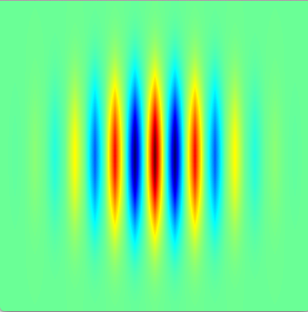
\includegraphics[scale=.4]{img/filter1.png}}
\quad
\subfloat[][Filter 2]{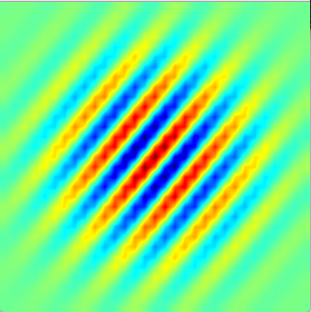
\includegraphics[scale=.4]{img/filter2.png}}

\caption{Two gabor filters.}
\label{fig:1}
\end{figure}
\begin{figure}
\centering
\subfloat[][Filter 1]{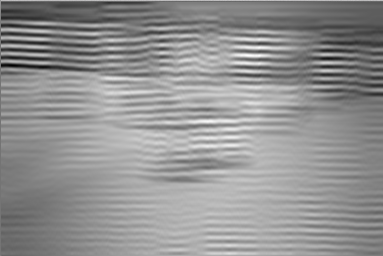
\includegraphics[scale=.35]{img/filteredImage1.png}}
\quad
\subfloat[][Filter 2]{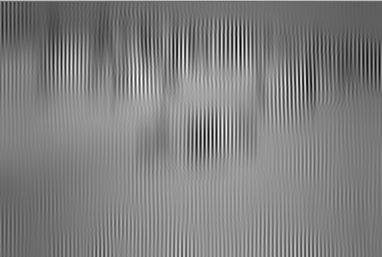
\includegraphics[scale=.35]{img/filteredImage2.png}}
\caption{An image of a beach scene (see Fig. \ref{fig:2} filtered with two different gabor filters. One of the filters had a horizontal orientation, the other one a vertical orientation, resulting in the highlighting of horizontal and vertical edges respectively.}

\label{fig:2}
\end{figure}

Each r*c feature vectors, each with 27 entries. We then generated distance maps displaying the euclidian distance of the feature vector of a reference pixel to all other feature vectors (see Figures \ref{fig:3}-\ref{fig:8}).


\begin{figure}
\centering
\subfloat[][Original Image]{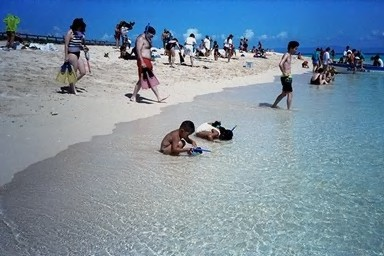
\includegraphics[scale=.25]{img/100.jpg}}
\quad
\subfloat[][Water Pixel]{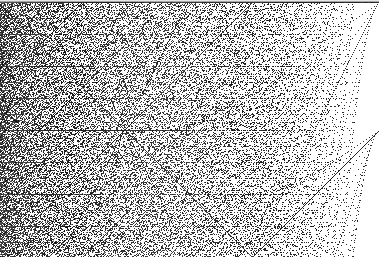
\includegraphics[scale=.25]{img/100water.png}}

\subfloat[][Person Pixel]{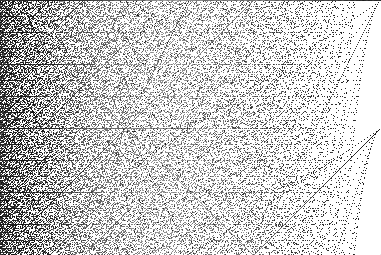
\includegraphics[scale=.25]{img/100person.png}}
\quad
\subfloat[][Sand Pixel]{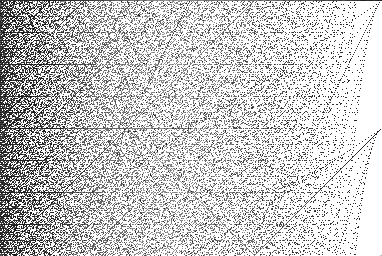
\includegraphics[scale=.25]{img/100sand.png}}
\caption{Image of a beach scene and three different distance maps. The captions indicate the approximate location of the reference pixels. }
\label{fig:3}
\end{figure}

\begin{figure}
\centering
\subfloat[][Original Image]{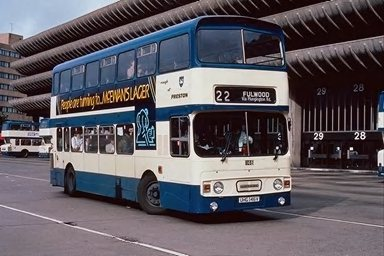
\includegraphics[scale=.25]{img/305.jpg}}
\quad
\subfloat[][Blacktop Pixel]{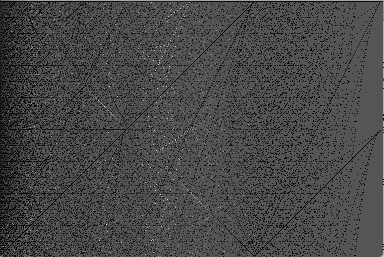
\includegraphics[scale=.25]{img/305blacktop.png}}

\subfloat[][White bus part pixel]{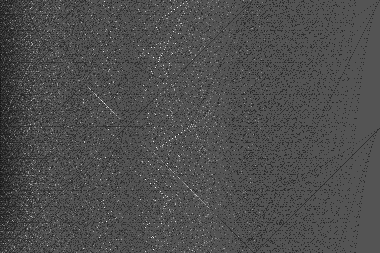
\includegraphics[scale=.25]{img/305white.png}}
\quad
\subfloat[][blue bus part pixel]{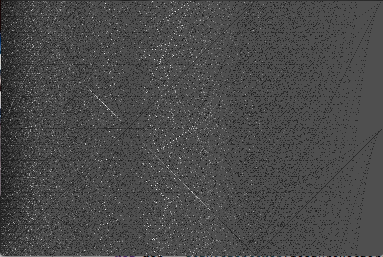
\includegraphics[scale=.25]{img/305blue.png}}
\caption{Image of a bus in a downtown area. }
\label{fig:4}
\end{figure}

\begin{figure}
\centering
\subfloat[][Original Image]{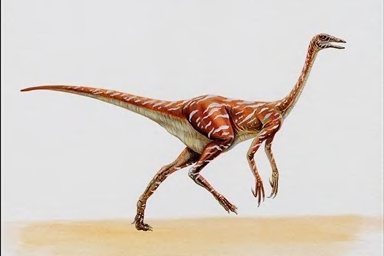
\includegraphics[scale=.25]{img/407.jpg}}
\quad
\subfloat[][Background pixel]{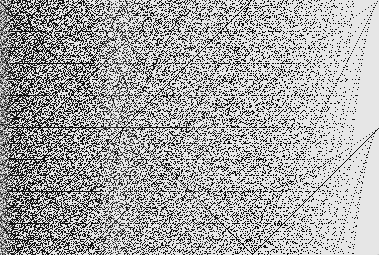
\includegraphics[scale=.25]{img/407backgrnd.png}}

\subfloat[][Brown body pixel]{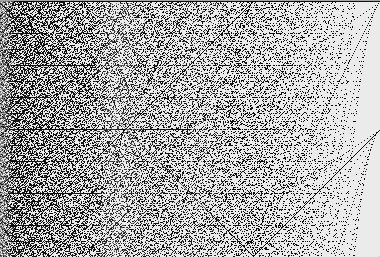
\includegraphics[scale=.25]{img/407brown.png}}
\quad
\subfloat[][White body pixel]{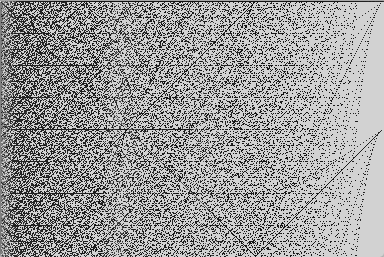
\includegraphics[scale=.25]{img/407whitebody.png}}
\caption{Image of a dinosaur painting.}
\label{fig:5}
\end{figure}

\begin{figure}
\centering
\subfloat[][Original Image]{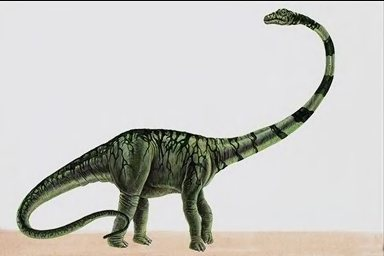
\includegraphics[scale=.25]{img/409.jpg}}
\quad
\subfloat[][Background pixel]{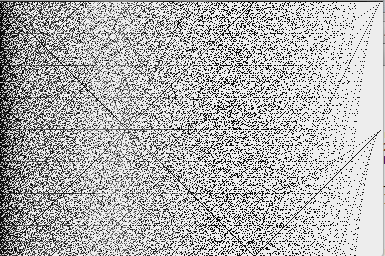
\includegraphics[scale=.25]{img/409backgrnd.png}}

\subfloat[][Body pixel]{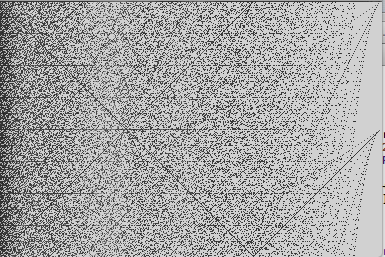
\includegraphics[scale=.25]{img/409body.png}}
\quad
\subfloat[][Head pixel]{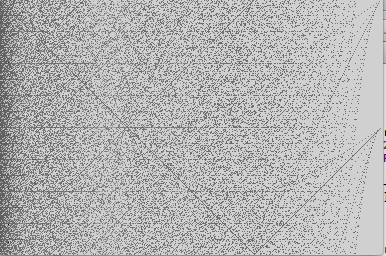
\includegraphics[scale=.25]{img/409head.png}}
\caption{Another dinosaur painting. }
\label{fig:6}
\end{figure}

\begin{figure}
\centering
\subfloat[][Original Image]{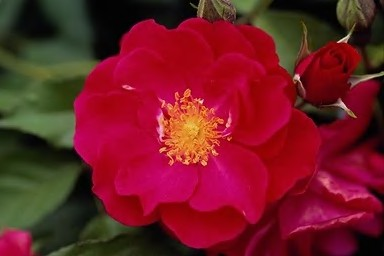
\includegraphics[scale=.25]{img/602.jpg}}
\quad
\subfloat[][Center flower pixel]{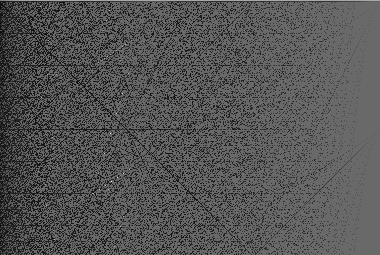
\includegraphics[scale=.25]{img/602middle.png}}

\subfloat[][Leaf pixel]{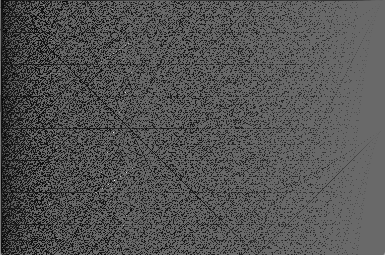
\includegraphics[scale=.25]{img/602green.png}}
\quad
\subfloat[][Petal pixel]{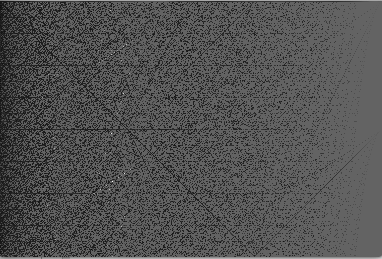
\includegraphics[scale=.25]{img/602bright.png}}
\caption{Image of a flower.}
\label{fig:7}
\end{figure}

\begin{figure}
\centering
\subfloat[][Original Image]{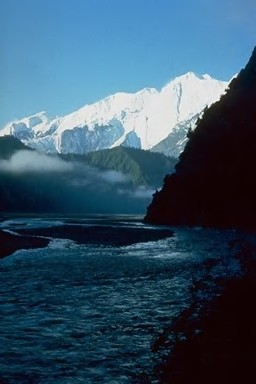
\includegraphics[scale=.45]{img/808.jpg}}
\quad
\subfloat[][Wood pixel]{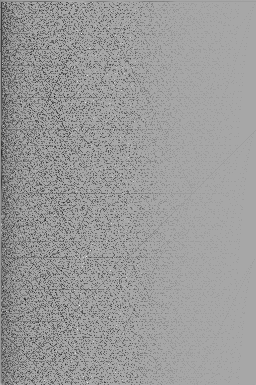
\includegraphics[scale=.45]{img/808green.png}}

\subfloat[][Snow pixel]{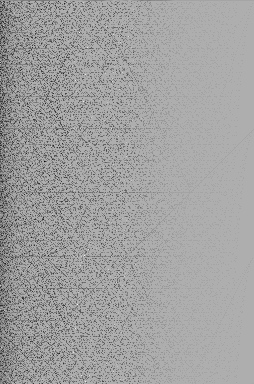
\includegraphics[scale=.45]{img/808snow.png}}
\quad
\subfloat[][Water pixel]{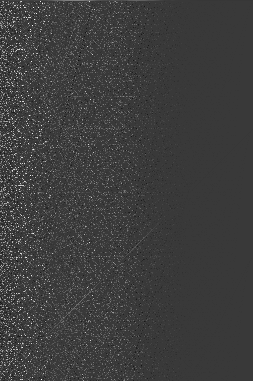
\includegraphics[scale=.45]{img/808water.png}}
\caption{Image of a mountain scene.}
\label{fig:8}
\end{figure}


\paragraph{Discussion}
For most of the selected images, the distance maps look surprisingly similar when comparing the three different pixels.
Exception: The mountain scene (Figure \ref{fig:8}

Some features are present across all the images, e.g. the lines crossing the center. These might be due to the chosen filter size and orientation.










\end{document}
